%!TEX root = ../MainBody.tex

\chapter{书写规范}
\section{文字、标点符号和数字}
汉字的使用应严格执行国家的有关规定,除特殊需要外,不得使用已废除的繁体字、异体字等不规范汉字。标点符号的用法应该以GB/T 15834—1995《标点符号用法》为准。数字用法应该以GB/T 15835—1995《出版物上数字用法的规定》为准。
\section{章节及各章标题}
论文正文须由另页右页开始。分章节撰写时每章也为另页右页开始,论文排版时注 意让每一章节的最后一页尽量不出现空白页面。各章标题中尽量不采用英文缩写词,尽 量不使用标点符号。
\section{序号}
\subsection{标题序号}
论文标题分层设序。层次以少为宜,根据实际需要选择。各层次标题一律用阿拉伯数字连续编号;不同层次的数字之间用小圆点“.”相隔,末位数字后面不加点号,如“1.1”,“1.1.1”等;章的标题居中排版,各层次的序号均左起顶格排,后空一个字距接排标题。例如:
\begin{figure}[!hbp]
    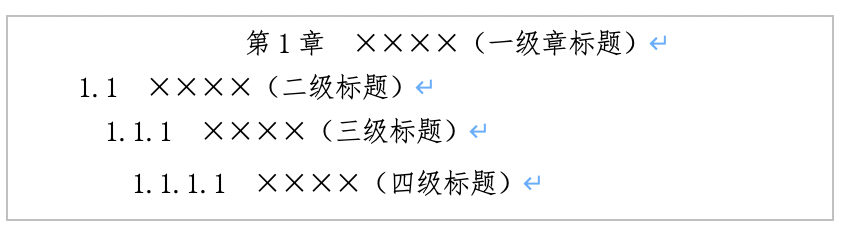
\includegraphics[width=13cm]{./Figures/levels}
    \centering
    \bicaption{图标题}{Title}
    \label{fig:levels}
\end{figure}
\subsection{图表等编号}
论文中的图、表、附注、公式、算式等,一律用阿拉伯数字分章依序连续编码。其 标注形式应便于互相区别,如:图 l.1(第 1 章第一个图)、图 2.2(第 2 章第二个图);3.2(第 3 章第二个表)等。
\subsection{页码}
页码从引言(或绪论)开始按阿拉伯数字(1,2,3……)连续编排,页码位于页 面下方居中、右页右下角;此前的部分(中、英文摘要、目录等)用大写罗马数字(I, II, III…)单独编排, 页码位于页面下方居中。
\subsection{页眉}
\section{名词和术语}
\section{量和单位}
\section{图和表}
\subsection{图}
插图须紧跟文述。在正文中,一般应先见图号及图的内容后再见图,一般情况下不能提前见图,特殊情况须延后的插图不应跨节;提供照片应大小适宜,主题明确,层次清楚,金相照片一定要有比例尺;图应具有“自明性”,即只看图、图题和图例,不阅读正文,就可理解图意。引用的图必须注明来源。

图的大小一般为宽6.67 cm×高5.00cm。特殊情况下,也可宽9.00 cm×高6.75cm,或宽13.5 cm×高9.00cm。同类图片的大小应尽量一致,编排美观、整齐。如\cref{fig:demo}
\begin{figure}[H]
    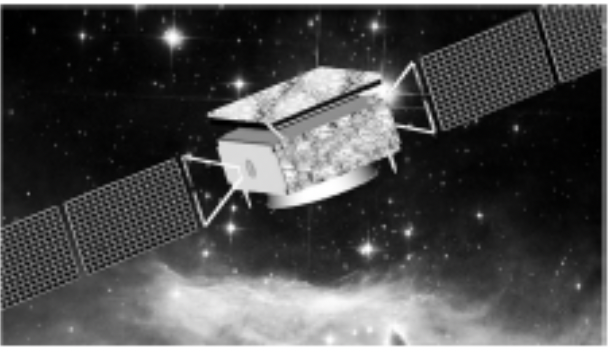
\includegraphics[width=9cm]{./Figures/demo}
    \centering
    \bicaption{图标题}{Title}
    \label{fig:demo}
\end{figure}
一幅图如有若干幅分图,均应编分图号,用(a),(b),(c),...... 按顺序编排,且各分图的分题注直接列在各自分图的正下方,总题注列在所有分图的下方正中。
\subsection{表}
表的编排一般是内容和测试项目由左至右横读,数据依序竖排,应有自明性,引用的表必须注明来源。具体要求如下:

每一表应有简短确切的题名,连同表序号置于表上居中。必要时,应将表中的符号、标记、代码及需说明的事项,以最简练的文字横排于表下作为表注。论文表的题名需用中文及英文两种文字表达,表注可用中英文两种文字表达或只用中文表达。

表内同一栏数字必须上下对齐。表内不应用“同上”、“同左”等类似词及“″”符号,一律填入具体数字或文字,表内“空白”代表未测或无此项,“—”或“…”(因“—”可能与代表阴性反应相混)代表未发现,“0”该表实测结果为零。

表格尽量用“三线表”,避免出现竖线,避免使用过大的表格,确有必要时可采用卧排表,正确方位应为“顶左底右”,即表顶朝左,表底朝右。表格太大需要转页时,需要在续表表头上方注明“续表”,表头也应重复排出。
表中用字为五号字体。如排列过密,用五号字有困难时,可小于五号字,但不小于七号。表格必须通栏,即表格宽度与正文版面平齐。
示例:
\begin{table}[htp]
    \bicaption{表标题}{Title}
	\centering
    % 调整表格,修改数字即可
    % \resizebox{\textwidth}{12mm}{ % 表格过宽
	\setlength{\tabcolsep}{1cm}{ %表格过窄
	\zihao{5}
	\begin{tabular}{cccc}
    \toprule
    文献类型  & 标志代码 & 文献类型 & 标志代码 \\
    \midrule
    普通图书  & M    & 会议录  & C    \\
    汇编    & G    & 报纸   & N    \\ 
    期刊    & J    & 学位论文 & D    \\
    报告    & R    & 标准   & S    \\
    专利    & P    & 数据库  & DB   \\
    计算机程序 & CP   & 电子公告 & EB   \\
    \bottomrule
    \end{tabular}}
    \label{tab:demo}    
\end{table}
\section{表达式(公式)}
论文中的公式应另起一行,居中编排,较长的公式尽可能在等号后换行,或者在“+”、“-”等符号后换行。公式中分数线的横线,长短要分清,主要的横线应与等号取平。公式后应注明编号,公式号应置于小括号中,如公式(2-3)。写在右边行末,中间不加虚线;公式下面的“式中:”两字左起顶格编排,后接符号及其解释;解释顺序为先左后右,先上后下;解释与解释之间用“;”隔开。

公式中各物理量及量纲均按国际标准(SI)及国家规定的法定符号和法定计量单位标注,禁止使用已废弃的符号和计量单位。
示例:
\begin{equation}
\label{eq:demo}
q=k_dH^x
\end{equation}
式中:q\cdash 灌水器流量/L·h-1;kd\cdash 流量系数;H\cdash 工作压力/m;x\cdash 流态指数。 

(此处,“式中:”改为顶格输出)

\section{算法(伪代码)}
本节介绍了一个伪代码示例,如\cref{alg:alg1}所示。
\begin{algorithm}
	\caption{Calculate $y = x^n$} 
	\label{alg:alg1}
	\begin{algorithmic}[1]
		% 输入
		\REQUIRE $n \geq 0 \vee x \neq 0$ 
		% 输出
		\ENSURE $y = x^n$ 
		
		% 初始化
		\STATE $y \leftarrow 1$ 
		
		% 逻辑
		\IF{$n < 0$} 
			\STATE $X \leftarrow 1 / x$ 
			\STATE $N \leftarrow -n$ 
		\ELSE 
			\STATE $X \leftarrow x$ 
			\STATE $N \leftarrow n$
		\ENDIF
		
		\WHILE{$N \neq 0$} 
			\IF{$N$ is even} 
				\STATE $X \leftarrow X \times X$ 
				\STATE $N \leftarrow N / 2$ 
			\ELSIF{$N$ is odd}
				\STATE $y \leftarrow y \times X$ 
				\STATE $N \leftarrow N - 1$ 
			\ENDIF 
		\ENDWHILE
	\end{algorithmic}
\end{algorithm}

\section{参考文献}
参照GB/T 7714—2015《信息与文献 参考文献著录规则》执行。
\section{附录}
附录编号依次为附录A,附录B。附录标题各占一行,按一级标题编排。每一个附录一般应另起一页编排,如果有多个较短的附录,也可接排。附录中的图、表、公式另行编排序号,与正文分开,编号前加“附录A-”字样。
附录作为主体部分的补充(不是必需的)。下列内容可作为附录编于论文后。

——为了整篇论文材料的完整,但编于正文又有损于编排的条理性和逻辑性,这一材料包括比正文更为详尽的信息、研究方法和技术更深入的叙述,以及对了解正文内容有用的补充信息等。

——由于篇幅过大或取材于复制品而不便于编入正文的材料。

——不便于编入正文的罕见珍贵资料。

——对一般读者并非必要阅读,但对本专业同行有参考价值的资料。

——正文中未被引用但被阅读或具有补充信息的文献。

——某些重要的原始数据、数学推导、结构图、统计表、计算机打印输出件等。
